\titleframe


%--------------------------------------------------------------------------------

\begin{frame}{Au dernier cours, nous avons vu}
\begin{itemize}
  \item Comment généraliser les concepts appris jusqu'à présent en utilisant la théorie des graphes appliquée à la PLK pour obtenir la méthode des n{\oe}uds
  \item Comment généraliser le théorème de Norton à $n-1$ accès, puis comment réduire ce modèle à $x<n-1$ accès
\end{itemize}

\end{frame}\begin{frame}{Qu'allons nous faire dans ce cours ?}
\begin{itemize}
  \item Apprendre une méthode duale à la méthode des n{\oe}uds : la méthode des mailles
  \item Généraliser le théorème de Thévenin pour des circuits à plusieurs accès
  \item utile lorsqu'on souhaite identifier les paramètres ou simplifier un modèle d'une partie d'un circuit "au milieu" d'autres parties.
\end{itemize}
\end{frame}

%--------------------------------------
% Table of contents
\begin{frame}{Plan du cours}
  \setbeamertemplate{section in toc}[sections numbered]
  \tableofcontents[hideallsubsections]
\end{frame}

%-------------------------------------------------------------------------------


\section{Théorie des graphes}
\begin{frame}{Branches, n{\oe}uds, graphes}
Une \textbf{branche} est\footnote{"Branch" ou "edge"en anglais} un segment de ligne dont les deux extrémités sont distinctes.

Un \textbf{n{\oe}ud} ou sommet\footnote{"Node" ou "vertex" en anglais.} est l'extrémité d'une branche (on admettra également qu'un n{\oe}ud peut être un point isolé.)

Un \textbf{graphe} $G$ est un ensemble de n{\oe}uds dont
certains sont reliés par des branches. On désigne par $n$ le nombre
de n{\oe}uds et par $b$ le nombre de branches.
\begin{center}
	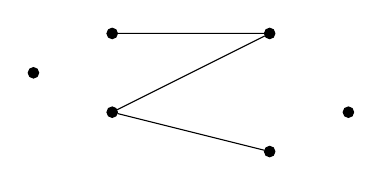
\begin{tikzpicture}
	\node[circle, draw, fill=black, scale = 0.4] (A) at (0,0) {};
	\node[circle, draw, fill=black, scale = 0.4] (B) at (2,0) {};
	\node[circle, draw, fill=black, scale = 0.4] (A2) at (0,-1) {};
	\node[circle, draw, fill=black, scale = 0.4] (B2) at (3,-1) {};
	\node[circle, draw, fill=black, scale = 0.4] (A3) at (-1,-.5) {};
	\node[circle, draw, fill=black, scale = 0.4] (B3) at (2,-1.5) {};
	\draw[black] (A) -- (B) -- (A2) -- (B3) ;
	\end{tikzpicture} \\ 
	Un graphe $G$ avec $n=6$ et $b=3$.
\end{center}

\end{frame} \begin{frame}{Orientation des branches}
Une \textbf{branche orientée} est une branche possédant une orientation fixée par
l'ordre des n{\oe}uds. Cette orientation est indiquée par une flèche pointant vers le second n{\oe}ud de la paire orientée. 

Par exemple, la fgure ci-dessous désigne la branche orientée $ab$.
Il est quelquefois utile de considérer seul le segment de ligne (branche sans ses extrémités), 
on parle alors d'\textbf{arc} si la branche à laquelle appartient le segment de ligne est orientée et d'\textbf{arête} si cette branche n'est pas orientée.
\begin{center}
	\begin{tikzpicture}
	\node[circle, draw, fill=black, scale = 0.4] (A) at (0,0) {};
	\node[circle, draw, fill=black, scale = 0.4] (B) at (2,0) {};
	\draw[arrows=-triangle 45,black] (A) node[above] {$a$} -- (B) node[above] {$b$} ;
	\node[circle, scale = 0.4] (A2) at (0,-0.5) {};
	\node[circle, scale = 0.4] (B2) at (2,-.5) {};
	\draw[arrows=-triangle 45,black] (A2) node[above] {$a$} -- (B2) node[above] {$b$} ;
	\node[circle, scale = 0.4] (A3) at (0,-1) {};
	\node[circle, scale = 0.4] (B3) at (2,-1) {};
	\draw[black] (A3)  node[above] {$a$} -- (B3) node[above] {$b$} ;
	\end{tikzpicture} \\
	{Branche orientée entre les n{\oe}uds $a$ et $b$, arc et arête.}
\end{center}

\end{frame} \begin{frame}{Graphe orienté}
Un graphe est orienté lorsque toutes ses branches le sont. 
Dans la théorie des circuits, seuls les graphes orientés nous intéressent.
\begin{center}
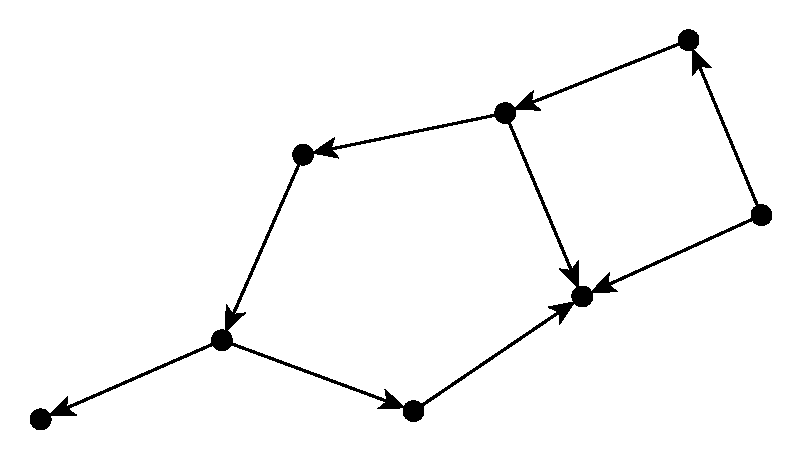
\includegraphics[width=0.5\linewidth]{figs/graphes/DG}
\end{center}
\end{frame} 

\begin{frame}{Sous-graphe}
Un sous-graphe d'un graphe est un sous-ensemble des branches
du graphe ; c'est lui-même un graphe. Il est dit "propre" s'il ne contient pas toutes les
branches du graphe dont il est issu.
\begin{center}
	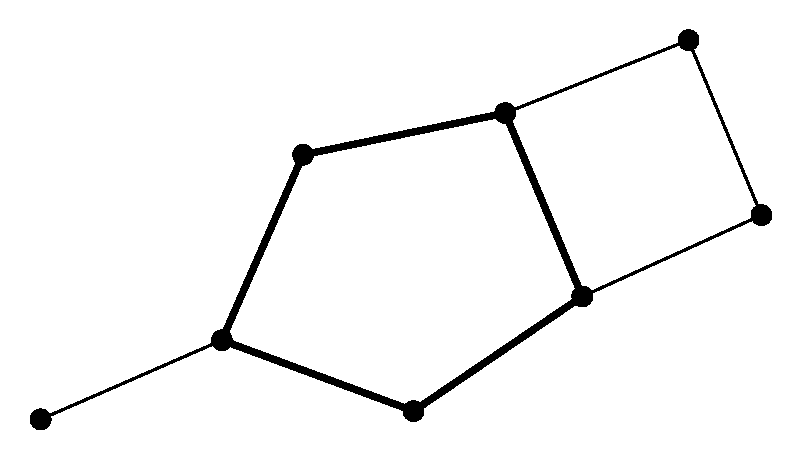
\includegraphics[width=0.5\linewidth]{figs/graphes/subgraph}\\
	{Sous graphe (arêtes en trait épais et n{\oe}uds incidents.)}
\end{center}

\end{frame} 

\begin{frame}{Incidence et chemin}
On dit qu'une branche $b$ est \textbf{incidente} à un n{\oe}ud $n$ si $n$ est une extrémité de $b$.

Un \textbf{parcours ou chemin}\footnote{Path en anglais.} est un sous-graphe d'un graphe composé
d'une suite ordonnée de branches dont chacune a un n{\oe}ud commun avec la branche précédente et l'autre n{\oe}ud commun avec la branche suivante et où chaque n{\oe}ud n'apparaît qu'une fois au plus.
\begin{center}
	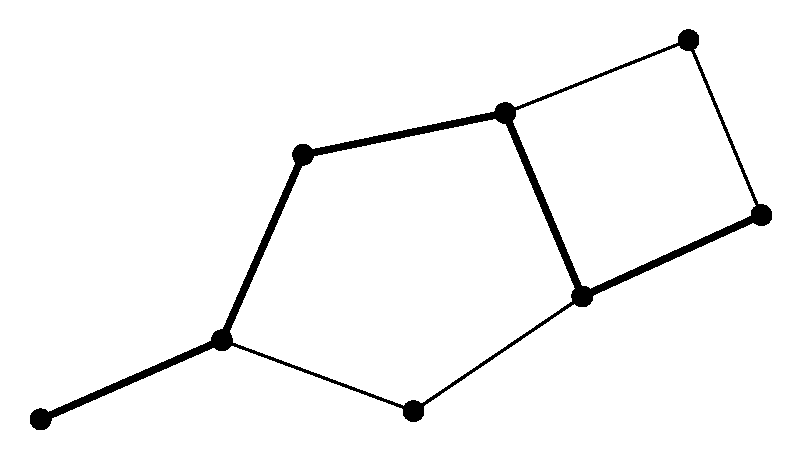
\includegraphics[width=0.4\linewidth]{figs/graphes/chemin}\\
	{Chemin (trait épais).}
\end{center}
\end{frame}

\begin{frame}{Degré, connexité}
Le \textbf{degré d'un n{\oe}ud.} est le nombre de branches incidentes à ce n{\oe}ud. Dans le graphe ci-dessus il y a $1$ n{\oe}ud de degré $1$, $4$ n{\oe}uds de degré $2$ et $3$ n{\oe}uds de degré $3$.

Un graphe est dit \textbf{connexe} (ou simplement connexe) s'il existe toujours un parcours entre deux quelconques de ses n{\oe}uds. Intuitivement un graphe est connexe s'il est d'une pièce. Sinon, il est appelé non-connexe ou multiplement connexe.
\begin{center}
	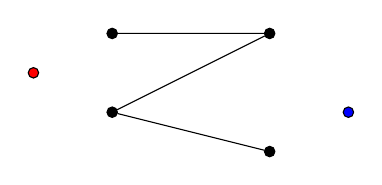
\begin{tikzpicture}
	\node[circle, draw, fill=black, scale = 0.4] (A) at (0,0) {};
	\node[circle, draw, fill=black, scale = 0.4] (B) at (2,0) {};
	\node[circle, draw, fill=black, scale = 0.4] (A2) at (0,-1) {};
	\node[circle, draw, fill=blue, scale = 0.4] (B2) at (3,-1) {};
	\node[circle, draw, fill=red, scale = 0.4] (A3) at (-1,-.5) {};
	\node[circle, draw, fill=black, scale = 0.4] (B3) at (2,-1.5) {};
	\draw[black] (A) -- (B) -- (A2) -- (B3) ;
	\end{tikzpicture} \\ 
	Graphe avec 3 composantes connexes.
\end{center}
\end{frame}

\begin{frame}[allowframebreaks]{La notion de maille}
  \begin{block}{Maille}
    Une maille (loop) est un sous-graphe connexe dont tous les n{\oe}uds sont de degré 2 (=cycle).
  \end{block}

\includegraphics[width=0.45\textwidth, center]{cbd435a9-cec2-4dd4-b13c-7b225dcc6548-06_694_1271_706_463}\\

\includegraphics[width=0.45\textwidth, center]{cbd435a9-cec2-4dd4-b13c-7b225dcc6548-06_694_1266_706_1824}\\

\includegraphics[width=0.45\textwidth, center]{cbd435a9-cec2-4dd4-b13c-7b225dcc6548-06_689_1257_1623_468}\\

\includegraphics[width=0.45\textwidth, center]{cbd435a9-cec2-4dd4-b13c-7b225dcc6548-06_694_1276_1618_1824}

\end{frame}\begin{frame}{Un arbre}
    \begin{block}{Arbre de recouvrement et maillons}
      Une \textit{arbre de recouvrement} est un sous-graphe connexe qui contient tous les n{\oe}uds du graphe initial et qui ne comporte aucune maille. 
      Les branches restantes non incluses dans l'arbre sont appelées \textit{maillons}.
      \begin{itemize}
        \item Nombre de branches de l'arbre pour un réseau connexe : $n-1$\\
        \item Nombre de maillons : $M = b-(n-1)$
      \end{itemize}
  \end{block}

\begin{columns}
  \begin{column}{0.45\textwidth}
  \begin{center}
  
\includegraphics[width=0.9\textwidth]{cbd435a9-cec2-4dd4-b13c-7b225dcc6548-07_696_1260_1227_350}
\end{center}
  \end{column}
  \begin{column}{0.45\textwidth}
    \#branches: 7\\
    \#maillons: 2
  \end{column}
\end{columns}
\end{frame}

\begin{frame}{Une maille fondamentale}
  \begin{block}{Maille fondamentale}
    Une \textit{maille fondamentale} est, pour un arbre donné, une maille formée à partir d'un seul maillon et de branches de l'arbre.
  \end{block}
  \begin{columns}
  \begin{column}{0.45\textwidth}
    
\includegraphics[width=0.8\textwidth, center]{cbd435a9-cec2-4dd4-b13c-7b225dcc6548-08_799_1266_735_291}
  \end{column}
  \begin{column}{0.45\textwidth}
    
\includegraphics[width=0.8\textwidth, center]{cbd435a9-cec2-4dd4-b13c-7b225dcc6548-08_684_1271_840_1700}\\
    
\includegraphics[width=0.8\textwidth, center]{cbd435a9-cec2-4dd4-b13c-7b225dcc6548-08_693_1267_1614_1704}
  \end{column}
\end{columns}
\end{frame}

\begin{frame}{Circuit et graphe}
On associe à un circuit un graphe orienté. L'orientation des branches est donnée par le sens du courant.

On se limite aux seuls graphes connexes.
On définit :
\begin{itemize}
  \item Etat électrique ou état : ( $\mathbf{u}_{B}(t), \mathbf{i}_{B}(t)$ ) ensemble des valeurs que prennent les courants et les tensions de branches à un instant donné
  \item $n$ : le nombre de n{\oe}uds du graphe ou du circuit
  \item $b$ : le nombre de branches
  \item le nombre de branches d'un arbre : $N=n-1$
  \item le nombre de maillons ou de mailles fondamentales : $M=b-(n-1)$
\end{itemize}
\end{frame}

\begin{frame}{Exemple}
  \begin{columns}
  \begin{column}{0.45\textwidth}
    \begin{center}
    
\includegraphics[width=0.5\textwidth]{cbd435a9-cec2-4dd4-b13c-7b225dcc6548-10_975_799_315_558}
    \end{center}
  \end{column}
  \begin{column}{0.45\textwidth}
    \begin{center}
      
\includegraphics[width=0.5\textwidth]{cbd435a9-cec2-4dd4-b13c-7b225dcc6548-10_994_908_253_2001}
    \end{center}
  \end{column}
\end{columns}

\begin{itemize}
  \item $n=5$,  $b=7$, $N=4$, $M=3$
  \item mailles : abdea , acea , acedba , . . . où face = abdea
  \item arbre : branches $1,2,3,4$ mailles fondamentales : abdea, bcedb, bacb maillons correspondants : 5,6,7
\end{itemize}
\end{frame}


\section{Méthode des mailles}
\begin{frame}{Méthode des mailles}
Pour déterminer l'état électrique d'un système, la méthode des mailles consiste à résoudre le système linéaire suivant (l'indice M signifie "Maille") : 
$$
\mathbf{R}_{\mathrm{M}} \mathbf{i}_{\mathrm{M}}=\mathbf{v}_{\mathrm{SM}}
$$

$\mathbf{i}_{\text {M }}$ est le vecteur des courants de maille
\begin{itemize}
  \item il contient les $b-(n-1)$ variables du système
\end{itemize} 
$\mathbf{V}_{s}$ M est le vecteur des sources indépendantes de tension agissant dans les mailles
\begin{itemize}
\item déterminé par inspection, il caractérise l'impact des sources indépendantes de tension.
  \item Les tensions de branches en découlent, via la loi d'Ohm\\
\end{itemize} 
$\mathbf{R}_{\mathrm{M}}$ est la matrice de résistances de mailles
\begin{itemize}
  \item déterminée par inspection ou par expérimentation, elle caractérise le graphe du circuit passifié
\end{itemize}

\begin{figure}[h]
\begin{center}
\captionsetup{labelformat=empty}
\caption{1. Choisir un arbre et orienter les branches}
  
\includegraphics[alt={},width=\textwidth]{cbd435a9-cec2-4dd4-b13c-7b225dcc6548-12_651_531_343_143}
\end{center}
\end{figure}

\begin{figure}[h]
\begin{center}
\captionsetup{labelformat=empty}
\caption{1. Choisir un arbre et orienter les branches}
  
\includegraphics[alt={},width=\textwidth]{cbd435a9-cec2-4dd4-b13c-7b225dcc6548-12_694_641_324_826}
\end{center}
\end{figure}

\begin{figure}[h]
\begin{center}
\captionsetup{labelformat=empty}
\caption{3. Déterminer $\mathbf{v}_{\mathrm{sM}}$}
  
\includegraphics[alt={},width=\textwidth]{cbd435a9-cec2-4dd4-b13c-7b225dcc6548-12_861_717_1384_396}
\end{center}
\end{figure}

$$
\mathbf{v}_{s \mathrm{M}}=(?, ?, ?)
$$

\begin{enumerate}
  \setcounter{enumi}{1}
  \item Déterminer $\mathbf{R}_{\mathrm{M}}$\\

\includegraphics[width=\textwidth, center]{cbd435a9-cec2-4dd4-b13c-7b225dcc6548-12_1019_1534_343_1843}
\end{enumerate}

\begin{figure}[h]
\begin{center}
  
\includegraphics[alt={},width=\textwidth]{cbd435a9-cec2-4dd4-b13c-7b225dcc6548-12_875_698_1384_1872}
\captionsetup{labelformat=empty}
\caption{$\dot{\mathbf{1}}_{\mathrm{M}}=\left(\dot{i}_{I}, \dot{i}_{I I}, \dot{i}_{I I I}\right)$}
\end{center}
\end{figure}

\end{frame}\begin{frame}{Conditions d'application}
\begin{itemize}
  \item Circuit linéaire
  \item Sources indépendantes de tension seulement
  \item Nous verrons plus tard comment gérer les sources indépendantes de courant et les source commandées de courant [CVT]
\end{itemize}

\everycircuitlink{https://everycircuit.com/circuit/6065539369795584}

\end{frame}\begin{frame}{Dérivation de la méthode des mailles}
\begin{center}
\begin{tabular}{lll}
(1) & $\mathbf{B u}_{\mathrm{B}}=\mathbf{v}_{\mathrm{s} \mathrm{M}}$ & SLK sur base de la matrice des mailles B \\
(2) & $\mathbf{i}_{\mathrm{B}}=\mathbf{B}^{\mathrm{T}} \mathbf{i}_{\mathrm{M}}$ & Définition des courants de branches à partir des courants de maille et de B \\
(3) & $\mathbf{u}_{\mathrm{B}}=\mathbf{R}_{\mathrm{B}} \mathbf{i}_{\mathrm{B}}$ & Loi d'Ohm, via la matrice de résistances de branches \\
(4) & $\mathbf{B R}_{\mathbf{B}} \mathbf{i}_{\mathbf{B}}=\mathbf{v}_{\mathrm{SM}}$ & (1) dans (3) \\
(5) & $\mathbf{B R}_{\mathrm{B}} \mathbf{B}^{\mathrm{T}} \mathbf{i}_{\mathrm{M}}=\mathbf{v}_{\mathrm{s} \mathrm{M}}$ & (2) dans (4) \\
(6) & $\mathbf{B R}_{\mathrm{B}} \mathbf{B}^{\mathrm{T}}=\mathbf{R}_{\mathrm{M}}$ & Définition de la matrice de résistances de mailles \\
(7) & $\mathbf{R}_{\mathrm{M}} \mathbf{i}_{\mathrm{M}}=\mathbf{v}_{\mathrm{SM}}$ & (5) dans (6): Résultat final \\
\end{tabular}
\end{center}
\end{frame}

\begin{frame}{La matrice des mailles $\mathbf{B}$}
Formulation duale à celle de la matrice d'incidence.\\
Repose sur l'utilisation :
\begin{itemize}
  \item de la SLK écrite pour $b-(n-1)$ mailles fondamentales
  \item de la matrice des mailles fondamentales du graphe du circuit qui caractérise les relations mailles-branches du circuit
\end{itemize}
\end{frame}
\begin{frame} {Seconde loi de Kirchhoff}
  \begin{columns}
  \begin{column}{0.45\textwidth}
    
\includegraphics[width=0.6\textwidth, center]{cbd435a9-cec2-4dd4-b13c-7b225dcc6548-16_1028_866_420_362}\\
  \end{column}
  \begin{column}{0.45\textwidth}
    
\includegraphics[width=0.6\textwidth, center]{cbd435a9-cec2-4dd4-b13c-7b225dcc6548-16_1062_1013_405_1805}
  \end{column}
\end{columns}
	$$
	{
		\begin{array}{rcccccccccl}
		I & :&  - u_1&     & + u_3  & +  u_4  & -  u_5 &    &    & = &
		0\\ 
		II & : &     & -u_2&+ u_3& +  u_4  &        &-  u_6  &        &
		= & 0\\
		III & : &  + u_1  &-  u_2&     &     &     &  & -  u_7 & = &
		0 \\
		IV & : & -  u_1  &+   u_2  &   &  & -    u_5   &+  u_6  &   
		& = & 0
		\end{array}}
	$$

\end{frame}

\begin{frame}{La matrice des mailles du graphe passifié}
  
$$
-\mathbf{B}_{a} \mathbf{u}_{B}=\mathbf{0} \quad \text { ou } \quad \mathbf{B}_{a} \mathbf{u}_{B}=\mathbf{0}
$$

$\mathbf{B}_{a}$ est la matrice des mailles du graphe orienté, d'ordre $m \times b$, obtenue comme suit :
\begin{itemize}
  \item $b_{i j}=+1 \quad$ si la branche $j$ appartient à la maille $i$ et est orientée dans le même sens
  \item $b_{i j}=-1 \quad$ si la branche $j$ appartient à la maille $i$ et est orientée en sens inverse
  \item $b_{i j}=0 \quad$ si la branche $j$ n'appartient pas à la maille $i$
\end{itemize}

$m$ est le nombre total de mailles du circuit (en général, il n'y pas d'expression analytique simple en fonction de $n$ et $b$).
Ce sont $m$ relations \alert{linéairement dépendantes} : par exemple (1)-(2) = (4)
\end{frame}

\begin{frame}
  \frametitle{Matrice des mailles fondamentales $\mathbf{B}$}
Si l'on choisit uniquement un ensemble de mailles fondamentales, on obtient $b-(n-1)$ relations indépendantes.

Soit $\mathbf{B}$ la matrice des mailles fondamentales :
\begin{columns}
  \begin{column}{0.45\textwidth}
    \begin{center}
      
\includegraphics[width=0.5\textwidth]{cbd435a9-cec2-4dd4-b13c-7b225dcc6548-18_1095_803_668_563}
    \end{center}
  \end{column}
  \begin{column}{0.45\textwidth}
    On a
    $$
    \mathbf{B}=\left[\begin{array}{rrrrrrr}
      1 & 0 & -1 & -1 & 1 & 0 & 0 \\
      0 & 1 & -1 & -1 & 0 & 1 & 0 \\
      -1 & 1 & 0 & 0 & 0 & 0 & 1
    \end{array}\right]
    $$
  \end{column}
\end{columns}

SLK sous forme matricielle : $\mathbf{B} \mathbf{u}_{B}=\mathbf{0}, b-(n-1)$ relations linéairement indépendantes.

\end{frame}

\begin{frame}{Vecteur $\mathbf{v}_{s \mathrm{M}}$}
  \begin{columns}
  \begin{column}{0.45\textwidth}
    \begin{center}
    
\includegraphics[width=\textwidth]{cbd435a9-cec2-4dd4-b13c-7b225dcc6548-19_808_1453_563_1155}
    \end{center}  
  \end{column}
  \begin{column}{0.45\textwidth}
    SLK dans les $b-(n-1)$ mailles fondamentales
    $$
    \begin{array}{lrl}
    I: & u_{1}-u_{3}+u_{5} & =-v_{s 1} \\
    II: & u_{2}-u_{3}+u_{6} & =-v_{s 1} \\
    III: & -u_{1}+u_{2}+u_{7} & =0
    \end{array} 
    $$
    $$ \Longleftrightarrow \mathbf{B} \mathbf{~ u}_{B}=\mathbf{v}_{s M} $$
  \end{column}
\end{columns}
\end{frame}


%B : matrice des mailles fondamentales du circuit passifié = circuit où l'on a rendues inactives toutes les sources indépendantes d'énergie.\\
%Sources indépendantes de tension, $v=0$ : remplacer par un court-circuit\\
%
\includegraphics[width=\textwidth, center]{cbd435a9-cec2-4dd4-b13c-7b225dcc6548-20_808_1123_926_210}

%$$
%\mathbf{B}=\left[\begin{array}{rrrrrr}
%1 & 0 & -1 & 1 & 0 & 0 \\
%0 & 1 & -1 & 0 & 1 & 0 \\
%-1 & 1 & 0 & 0 & 0 & 1
%\end{array}\right]
%$$

\begin{frame}
  \frametitle{Courants de mailles}

  Vecteur $\mathbf{i}_{M}$ des courants dans les maillons : $\mathbf{i}_{M}=\left[i_{5}, i_{6}, i_{7}\right]^{T}$.

\begin{columns}
  \begin{column}{0.45\textwidth}
    
\includegraphics[width=0.6\textwidth, center]{cbd435a9-cec2-4dd4-b13c-7b225dcc6548-21_1109_813_702_210}
  \end{column}
  \begin{column}{0.45\textwidth}
  $$
  \left[\begin{array}{l}
    i_{1} \\
    i_{2} \\
    i_{3} \\
    i_{4} \\
    i_{5} \\
    i_{6} \\
    i_{7}
  \end{array}\right]=\left[\begin{array}{rrr}
    1 & 0 & -1 \\
    0 & 1 & 1 \\
    -1 & -1 & 0 \\
    -1 & -1 & 0 \\
    1 & 0 & 0 \\
    0 & 1 & 0 \\
    0 & 0 & 1
  \end{array}\right]\left[\begin{array}{c}
    i_{I} \\
    i_{I I} \\
    i_{I I I}
  \end{array}\right]
  $$
  \end{column}
\end{columns}
  
  PLK sous forme matricielle : $\mathbf{i}_{B}=\mathbf{B}^{T} \mathbf{i}_{M}$.
\end{frame}
  
\begin{frame}{Matrices de résistances de mailles $\mathbf{R}_{\mathrm{M}}$}
Appliquer la loi d'Ohm dans chaque branche (relation $u=f(i)$ ) permet de remplacer $\mathbf{u}_{B} \operatorname{par} \mathbf{i}_{B}$

$$
\begin{aligned}
u_{1}=R_{1} i_{1}, \quad u_{2}=R_{2} i_{2}, & \ldots, \quad u_{7}=R_{7} i_{7} \\
R_{1} i_{1}-R_{3} i_{3}+R_{5} i_{5} & =-v_{s 1} \\
R_{2} i_{2}-R_{3} i_{3}+R_{6} i_{6} & =-v_{s 1} \quad \Longleftrightarrow \quad \mathbf{u}_{B}=\mathbf{R}_{B} \mathbf{i}_{B} \\
-R_{1} i_{1}+R_{2} i_{2}+R_{7} i_{7} & =0
\end{aligned}
$$

$\mathbf{R}_{B}$ : matrice de résistances de branches

$$
\mathbf{R}_{B}=\left[\begin{array}{cccc}
R_{1} & & & \\
& R_{2} & \mathbf{0} & \\
& \mathbf{0} & \ddots & \\
& & & R_{7}
\end{array}\right] \quad \begin{aligned}
& \text { matrice diagonale si résistances} \\
& \text { linéaires uniquement }
\end{aligned}
$$
\end{frame}

\begin{frame}{Remplacer les courants de branches $\mathbf{i}_{B}$ par les courants de mailles $\mathbf{i}_{M}$ via la PLK}
$$
\begin{aligned}
i_{1}=i_{M 1}-i_{M 3} \quad i_{2}=i_{M 2}+i_{M 3} \quad \ldots \quad i_{7}=i_{M 3} & \Longleftrightarrow \mathbf{i}_{B}=\mathbf{B}^{T} \mathbf{i}_{M} \\
\left(R_{1}+R_{3}+R_{5}\right) i_{M 1}+R_{3} i_{M 2}-R_{1} i_{M 3} & =-v_{s 1} \\
R_{3} i_{M 1}+\left(R_{2}+R_{3}+R_{6}\right) i_{M 2}+R_{2} i_{M 3} & =-v_{s 1} \\
-R_{1} i_{M 1}+R_{2} i_{M 2}+\left(R_{1}+R_{2}+R_{7}\right) i_{M 3} & =0 \\
\Longleftrightarrow &
\end{aligned}
$$

$$
\underbrace{\mathbf{B R}_{B} \mathbf{B}^{T}}_{\mathbf{R}_{M}} \mathbf{i}_{M}=\mathbf{v}_{s M}
$$

\end{frame}

\begin{frame}{Matrice de résistances de mailles}
  On obtien finalement 
$$
\mathbf{R}_{M}=\mathbf{B} \mathbf{R}_{B} \mathbf{B}^{T}=\left[\begin{array}{ccc}
R_{1}+R_{3}+R_{5} & R_{3} & -R_{1} \\
R_{3} & R_{2}+R_{3}+R_{6} & R_{2} \\
-R_{1} & R_{2} & R_{1}+R_{2}+R_{7}
\end{array}\right]
$$

\begin{center}

\includegraphics[width=0.5\textwidth]{cbd435a9-cec2-4dd4-b13c-7b225dcc6548-24_813_1462_649_1041}
\end{center}

\end{frame}\begin{frame}{Détermination de $\mathbf{R}_{M}$ par inspection}
\begin{itemize}
  \item $R_{i i}=$ somme des résistances des branches de la maille $i$
  \item $R_{i k}=$ somme des résistances des branches communes aux mailles $i$ et $k$, prises avec le signe + si les sens de parcours des deux mailles coïncident, avec le signe dans le cas contraire
\end{itemize}

\end{frame}

\begin{frame}{Application à notre exemple}
  

  $$
  \mathbf{R}_{M}= \left[\begin{array}{ccc}
3 & 1 & -1 \\
1 & 3 & 1 \\
-1 & 1 & 3
\end{array}\right]
$$

$$\mathbf{v}_{s M} = (-12, -12, 0)$$
On obtient $$\mathbf{i}_{M} = {\bf R}_M^{-1}\mathbf{v}_{sM} =  (-3, -3, 0) \text{ A}$$ qui se vérifie ici:
\everycircuitlink{https://everycircuit.com/circuit/6065539369795584}
\end{frame}




\begin{frame}{Réseau équivalent}
Le circuit peut être remplacé par un circuit équivalent constitué du circuit passifié vu de $M=b-(n-1)$ accès auquels agissent des sources indépendantes de tension équivalentes regroupant les sources indépendantes du circuit original.

\begin{columns}
  \begin{column}{0.45\textwidth}
    
\includegraphics[width=0.8\textwidth, center]{cbd435a9-cec2-4dd4-b13c-7b225dcc6548-25_894_1376_955_181}
  \end{column}
  \begin{column}{0.45\textwidth}
    Réseau passifié avec
    \begin{itemize}
      \item un accès dans chaque maillon (on "ouvre" le maillon)
      \item une source indépendante de tension agissant à chaque accès qui "ferme" le maillon
    \end{itemize}
  \end{column}
\end{columns}
\end{frame}

\begin{frame}{Exemple}
\begin{center}

\includegraphics[width=0.7\textwidth]{cbd435a9-cec2-4dd4-b13c-7b225dcc6548-26_1376_2671_525_85}
\end{center}

\end{frame}

\begin{frame}[allowframebreaks]{Et si le circuit comporte des sources commandées ?}
Source de type CVT uniquement, introduit une relation de branche du type $u=f(i)$, donc change la matrice $\mathbf{R}_B$\footnote{Autres types de sources commandées : pas toujours possible}
\begin{columns}
  \begin{column}{0.45\textwidth}
    
\includegraphics[width=\textwidth, center]{cbd435a9-cec2-4dd4-b13c-7b225dcc6548-27_818_1462_907_1041}
    $$
    \text { relation } u=f(i): \quad u_{1}=r_{m} i_{6}=r_{m} i_{M 2}
    $$
  \end{column}
  \begin{column}{0.45\textwidth}
    SLK dans la maille $\mathrm{I}: R_{3}\left(i_{M 1}+i_{M 2}\right)+R_{5} i_{M 1}+r_{m} i_{M 2}=-v_{s 1}$\\
    SLK dans la maille III : $R_{2}\left(i_{M 2}+i_{M 3}\right)+R_{7} i_{M 3}-r_{m} i_{M 2}=0$
  \end{column}
\end{columns}

    Matrice de résistances de branches :
    $$
    \mathbf{R}_{B}=\left[\begin{array}{cccccc}
    0 & 0 & 0 & 0 & r_{m} & 0 \\
    0 & R_{2} & 0 & 0 & 0 & 0 \\
    0 & 0 & R_{3} & 0 & 0 & 0 \\
    0 & 0 & 0 & R_{5} & 0 & 0 \\
    0 & 0 & 0 & 0 & R_{6} & 0 \\
    0 & 0 & 0 & 0 & 0 & R_{7}
    \end{array}\right]
    $$  

    Matrice de résistances de mailles :
    $$
    \mathbf{R}_{M}=\mathbf{B} \mathbf{R}_{B} \mathbf{B}^{T}=\left[\begin{array}{ccc}
    R_{3}+R_{5} & R_{3}+r_{m} & 0 \\
    R_{3} & R_{2}+R_{3}+R_{6} & R_{2} \\
    0 & R_{2}-r_{m} & R_{2}+R_{7}
    \end{array}\right]
    $$
    
    Même matrice B que précédemment.

\begin{itemize}
  \item $\mathbf{R}_{B}$ et $\mathbf{R}_{M}$ ne sont plus des matrices symétriques. 
  \item $\mathbf{R}_{M}$ ne peut plus être déterminée par inspection !!
\end{itemize}
\end{frame}

\begin{frame}{Si il y a des sources indépendantes de courant}
\begin{itemize}
  \item source en parallèle avec une résistance : transformer la source de courant en une source de tension équivalente
  \item source seule dans une branche : transformer le circuit de la manière suivante
\end{itemize}

\begin{columns}
  \begin{column}{0.45\textwidth}
  
\includegraphics[width=0.45\textwidth, center]{cbd435a9-cec2-4dd4-b13c-7b225dcc6548-35_827_1071_1022_372}\\
  \end{column}
  \begin{column}{0.45\textwidth}
  
\includegraphics[width=0.45\textwidth, center]{cbd435a9-cec2-4dd4-b13c-7b225dcc6548-35_1003_1171_936_1604}
  \end{column}
\end{columns}

On vérifie que dans le reste du circuit, les LK sont inchangées.\\
!! La branche dans laquelle se trouve la source ne doit pas être couplée avec le reste du circuit (par une source commandée par exemple)

\end{frame}

\section{Méthode d'expérimentation}
\begin{frame}{Principe}
Utiliser le réseau équivalent; $\mathbf{R}_{M}$ caractérise le circuit passifié. Les relations $u-i$ aux $b-(n-1)$ accès s'écrivent :
$$
\begin{aligned}
& u_{1}=R_{11} i_{1}+R_{12} i_{2}+\ldots \\
& u_{2}=R_{21} i_{1}+R_{22} i_{2}+\ldots
\end{aligned}
$$

i est le vecteur des courants injectés aux accès, $\mathbf{v}$ est le vecteur des tensions aux accès.
\end{frame}

\begin{frame}{Détermination de la matrice de résistance de mailles par expérimentation}
Les éléments de $\mathbf{R}_{M}$ sont déterminés par des essais successifs :
$$
R_{i j}=\left.u_{i}\right|_{i_{j}=1, i_{k}=0, k \neq j}
$$
\begin{itemize}
  \item Imposer un courant de 1 A à l'accès $j$
  \item Laisser les autres accès ouverts ( $i=0$ )
  \item Déterminer dans ces conditions la tension à l'accès $i$
\end{itemize}
\end{frame}

\begin{frame}{Elément diagonal}

\includegraphics[width=0.4\textwidth, center]{cbd435a9-cec2-4dd4-b13c-7b225dcc6548-30_918_1425_678_386}
$$
R_{i i}=\left.v_{i}\right|_{i_{i}=1, i_{k}=0, k \neq i}
$$

Tension à l'accès $i$ lorsque tous les accès sauf l'accès $i$ sont laissés ouverts.

\end{frame}

\begin{frame}{Elément non-diagonal}

\includegraphics[width=0.4\textwidth, center]{cbd435a9-cec2-4dd4-b13c-7b225dcc6548-31_913_1425_678_386}
$$
R_{i j}=\left.v_{i}\right|_{i_{j}=1, i_{k}=0, k \neq j}
$$

Tension à l'accès $i$ lorsque tous les accès sauf l'accès $j$ sont laissés ouverts.

\end{frame}

\begin{frame}[allowframebreaks]{Exemple}
  \begin{columns}
  \begin{column}{0.45\textwidth}
    $$
    R_{11}=\left.v_{I}\right|_{i_{I}=1, i_{I I}=i_{I I I}=0}
    $$
    \begin{center}
    
\includegraphics[width=0.8\textwidth]{cbd435a9-cec2-4dd4-b13c-7b225dcc6548-32_1353_1362_601_659}
    \end{center}  
  \end{column}
  \begin{column}{0.45\textwidth}
    $$
    \begin{aligned}
    i_{6} & =0 \\
    R_{11}=v_{I} & =R_{5}+R_{3}
    \end{aligned}
    $$
  \end{column}
\end{columns}

\begin{columns}
  \begin{column}{0.45\textwidth}
    $$
    R_{12}=\left.v_{I}\right|_{i_{I I}=1, i_{I}=i_{I I I}=0}
    $$
    \begin{center}
    
\includegraphics[width=0.8\textwidth]{cbd435a9-cec2-4dd4-b13c-7b225dcc6548-33_1353_1329_601_692}
    \end{center}
  \end{column}
  \begin{column}{0.45\textwidth}
    $$
    \begin{aligned}
    i_{5} & =0 \\
    i_{6} & =1 \\
    R_{12}=v_{I} & =R_{3}+r_{m}
    \end{aligned}
    $$
  \end{column}
\end{columns}

\begin{columns}
  \begin{column}{0.45\textwidth}  
    $$
    R_{13}=\left.v_{I}\right|_{i_{I I I}=1, i_{I}=i_{I I}=0}
    $$
    \begin{center}
    
\includegraphics[width=0.8\textwidth]{cbd435a9-cec2-4dd4-b13c-7b225dcc6548-34_1358_1481_448_616}
    \end{center}
  \end{column}
  \begin{column}{0.45\textwidth}
    $$
    \begin{gathered}
    i_{6}=0 \\
    R_{13}=v_{I}=0
    \end{gathered}
    $$
  \end{column}
\end{columns}


Exercice : appliquer la méthode expérimentale pour déterminer les éléments de la matrice $\mathbf{R}_{M}$ et en déduire la règle de calcul par inspection.
\end{frame}

\section{Théorème de Thévenin généralisé}

\begin{frame}[allowframebreaks]{Théorème de Thévenin généralisé à plusieurs accès}
  \begin{columns}
  \begin{column}{0.45\textwidth}
    À partir du schéma équivalent du circuit déduit de la méthode des mailles, en considérant $M=b-(n-1)$ accès, on ouvre chaque maillon pour y placer un accès.\\
  \end{column}
  \begin{column}{0.45\textwidth}
    
\includegraphics[width=0.9\textwidth, center]{cbd435a9-cec2-4dd4-b13c-7b225dcc6548-36_1003_1526_843_209}
  \end{column}
\end{columns}

\begin{columns}
  \begin{column}{0.45\textwidth}
  Les relations $u-i$ pour les $M$ accès sont : 
$$
\begin{aligned}
\mathbf{u} & =-\mathbf{v}_{s M}+\mathbf{R}_{M} \mathbf{i}_{M} \\
\mathbf{u} & =-\mathbf{v}_{s M}+\mathbf{R}_{M} \mathbf{i}
\end{aligned}
$$
  \end{column}
  \begin{column}{0.45\textwidth}
Le schéma équivalent de Thévenin à $M$ accès est obtenu en identifiant que
$$
\mathbf{v}_{T h}=-\mathbf{v}_{s M}, \quad \mathbf{R}_{T h}=\mathbf{R}_{M}
$$
  \end{column}
\end{columns}
\end{frame}

\begin{frame}{Exemple}
\begin{center}

\includegraphics[width=0.7\textwidth]{cbd435a9-cec2-4dd4-b13c-7b225dcc6548-37_1758_3177_463_23}
\end{center}
\end{frame}

\begin{frame}{Réduction du nombre d'accès}

Soit $a < M$ le nombre d'accès \alert{intéressants} (a) (desquels on observe le circuit). 
Les accès \textbf{inintéressants} sont court-circuités de manière à préserver la topologie du circuit. (b)
$$
u_{a+1}, \ldots, u_{M}=0
$$

\begin{center}

\includegraphics[width=0.4\textwidth]{cbd435a9-cec2-4dd4-b13c-7b225dcc6548-38_1004_1629_1002_907}
\end{center}
\end{frame}

\begin{frame}{Partitionnement}
On partitionne les relations $u-i$ de la méthode des mailles comme suit :
$$
\begin{gathered}
{\left[\begin{array}{c}
\mathbf{u}_{\mathbf{a}} \\
\mathbf{u}_{\mathbf{b}}
\end{array}\right]=-\left[\begin{array}{c}
\mathbf{v}_{s \mathbf{a}} \\
\mathbf{v}_{s \mathbf{b}}
\end{array}\right]+\left[\begin{array}{ll}
\mathbf{R}_{\mathbf{a}, \mathbf{a}} & \mathbf{R}_{\mathbf{a}, \mathbf{b}} \\
\mathbf{R}_{\mathbf{b}, \mathbf{a}} & \mathbf{R}_{\mathbf{b}, \mathbf{b}}
\end{array}\right]\left[\begin{array}{c}
\mathbf{i}_{\mathbf{a}} \\
\mathbf{i}_{\mathbf{b}}
\end{array}\right]} \\
\end{gathered}
$$
Comme $\mathbf{u}_{\mathbf{b}}=0=-\mathbf{v}_{s \mathbf{b}}+\mathbf{R}_{\mathbf{b}, \mathbf{a}} \mathbf{i}_{\mathbf{a}}+\mathbf{R}_{\mathbf{b}, \mathbf{b}} \mathbf{i}_{\mathbf{b}} \rightarrow \mathbf{i}_{\mathbf{b}}=\mathbf{R}_{\mathbf{b}, \mathbf{b}}^{-1}\left(\mathbf{v}_{s \mathbf{b}}-\mathbf{R}_{\mathbf{b}, \mathbf{a}} \mathbf{i}_{\mathbf{a}}\right)$, \\
on a $\mathbf{u}_{\mathbf{a}}=\left(-\mathbf{v}_{s \mathbf{a}}+\mathbf{R}_{\mathbf{a}, \mathbf{b}} \mathbf{R}_{\mathbf{b}, \mathbf{b}}^{-1} \mathbf{v}_{s \mathbf{b}}\right)+\left(\mathbf{R}_{\mathbf{a}, \mathbf{a}}-\mathbf{R}_{\mathbf{a}, \mathbf{b}} \mathbf{R}_{\mathbf{b}, \mathbf{b}}^{-1} \mathbf{R}_{\mathbf{b}, \mathbf{a}}\right) \mathbf{i}_{\mathbf{a}}$. \\
Finalement :
$$
\mathbf{u}_{\mathbf{a}}=\mathbf{v}_{T h}+\mathbf{R}_{T h} \mathbf{i}_{\mathbf{a}}
$$

\end{frame}

\begin{frame}{Paramètres du schéma équivalent}
Vecteur des sources équivalentes de Thévenin :

$$
\mathbf{v}_{T h}=-\mathbf{v}_{s \mathbf{a}}+\mathbf{R}_{\mathbf{a}, \mathbf{b}} \mathbf{R}_{\mathbf{b}, \mathbf{b}}^{-1} \mathbf{v}_{s \mathbf{b}}
$$

$=$ vecteur des tensions aux bornes des accès à vide ( $\mathbf{i}_{\mathbf{a}}=\mathbf{0}$ )\\
Matrice de résistances de Thévenin = matrice de résistances "réduite" aux accès :

$$
\mathbf{R}_{T h}=\mathbf{R}_{\mathbf{a}, \mathbf{a}}-\mathbf{R}_{\mathbf{a}, \mathbf{b}} \mathbf{R}_{\mathbf{b}, \mathbf{b}}^{-1} \mathbf{R}_{\mathbf{b}, \mathbf{a}}
$$

Peut être déterminée par expérimentation mais jamais par inspection

\end{frame}